
    The Compiler Analysis Description Language (CAnDL)
    makes the constraint methodology introduced in
    \Cref{chapter:theory}
    directly available to the LLVM infrastructure and the Clang compiler.
    The previous chapter showed how this enables powerful compiler analysis
    generation for many established compiler analysis tasks,
    from reimplementing peephole optimisations to detecting well-behaved code
    suitable for polyhedral analysis.

    This chapter uses CAnDL to go beyond established analysis methods and
    implement novel detection functionality to enable the automatic
    parallelisation of a wide class of programs.
    The previously overlooked ``complex reduction and histogram computations''
    are identified as an important class of parallelisation opportunities that
    are not accessible via conventional analysis approaches.
    Complex reductions and histogram computations may contain indirect memory
    access and kernel computations with non-trivial control flow.

    Complex reduction and histogram computations were not previously
    interpreted as a single class of calculations.
    Instead, the focus was on simpler scalar reductions, with no connection to
    histograms.
    However, this chapter demonstrates that several standard benchmark programs
    are dominated by loops that can be classified as complex reduction and
    histogram computations.
    Furthermore, they can be parallelised in the same way, by privatising scalar
    reduction variables and histogram reduction arrays.
    This allows for the automatic parallelisation of programs that were
    previously largely inaccessible to compiler analysis.

    By grouping complex reductions and histogram computations together and
    formulating them in CAnDL, a completely automatic detection in C/C++ code is
    possible.
    Parallelisation routines are then implemented to complement the detection.
    Well-established parallelisation approaches then result in good speedups on
    several relevant programs.
    This was evaluated on the NAS parallel benchmark suite as well as the
    Parboil benchmarks.

\section{Introduction}

    Reductions occur widely in numerical applications, and there are established
    techniques for parallelising them \citep{Jradi2017fast}.
    Typical reductions successively apply an arithmetic operator to an
    array of numeric values, in order to compute, for example, the sum of a set
    of floating point numbers.
    Perhaps most prominently, a reduction features in the innermost loop of the
    matrix multiplication kernel in the form of a dot product.
    In this form, reductions are critical to many high performance computing
    (HPC) workloads based on linear algebra, as well as embedded benchmarks and
    emerging machine learning and computer vision applications
    \citep{Reddy2016Reduction}.

    However, there is a much larger class of computations that can be
    interpreted as reductions than these scalar computations, and this class
    consitutes another important set of common kernels.
    The computations that this chapter will investigate include irregular
    reductions and histograms.
    Such reductions are typically more intense computationally and can be
    more profitably exploited on their own.

    Discovering and exploiting scalar reductions in programs has been
    studied for many years, among others by \citet{pottenger1995idiom}.
    The treatment of generalisations of reduction operations has received less
    attention.
    While some work has been published on parallelising such computations,
    automatic detection mostly evades the common compiler analysis methods.
    The reason is that histogram reductions intrinsically contain indirect
    memory accesses, which poses a challenge to compilers that use
    data dependence \citep{kuck1981dependence} or polyhedral
    representation \citep{benabderrahmane2010polyhedral} as the basis for
    their analysis.

%    Most prior work has focused on the exploitation of generalised reductions
%    rather than discovery.
%    Among this work, \citet{yu2006adaptive} examined performance trade-offs in
%    implementations, and \citet{Huo2011HiPC} studied the exploitation of novel
%    hardware.
%    Early work focused on well structured Fortran and paid little attention to
%    compiler-based detection.
%    More recent work by \citet{Han2010Speculative} has attempted to find
%    reductions in more complex C based code with partial reduction variables.
%    This approach is  based on update chains in the dependence graph and
%    requires hardware speculation support to check dependences, but is unable to
%    detect histogram reductions.
%    In \cite{Johnson:2012:SSP:2254064.2254107}, a complex system is
%    proposed to allow structure privatization, yet it only exploits simple
%    scalar reductions.
%    The difficulty in automatically detecting reductions has led to language or
%    annotation based approaches where it is the user's responsibility to mark
%    reductions in the program \cite{Reddy2016Reduction,ciesko2015scaling}.
%
    This chapter develops a new compiler based approach that automatically
    detects a wide class of generalised reductions.
    Such reductions can span large sections of code, contain general
    control-flow, have non-linear access to arrays and include histograms.
    Rather than developing a bespoke detection pass, the methodology is based on
    the previously introduced CAnDL constraint programming language.
    This formulation allows us to specify the reduction idiom using data flow
    and control flow constraints.
    During compilation, the CAnDL solver automatically identifies
    subsets within LLVM IR that constitute a reduction operation.

    The chapter focuses on the detection of reductions and then assumes later
    compiler stages are responsible for mapping to existing tuned libraries.
    However, to illustrate the potential performance of the scheme, a code
    generation pass was implemented that generates templated parallel pthread
    reduction code.
    This transformation pass achieved significant speedups on those benchmarks
    where reductions are performance bottlenecks.

    The approach was applied to C/C++ versions of three well known benchmark
    suites:
    NAS \cite{seo2011performance},
    Parboil \cite{stratton2012parboil} and
    Rodinia \cite{Che2009Rodinia}.
    These are non-trivial code bases and vary considerably in terms of code
    structure and complexity.
    State-of-the-art polyhedral and data dependence approaches are compared
    against.
    None of them find general histogram reductions, whereas the CAnDL approach
    detects 84 scalar reductions and 6 histograms.
    %% In order to further evaluate our approach, we manually profiled and
    %% examined the code and found that our approach is able to determine xyz\% of 
    %% all possible reductions.

%    Our constraint based approach can be used for a wide range of optimizations 
%    beyond reduction detection.
%    To illustrate this we prototyped a linear algebra kernel detection pass
%    which replaces dense and sparse matrix operations with the appropriate
%    library call leading to significant speedup.
%
%    This paper makes the following contributions:
%
%    \begin{itemize}
%    \item Detection of more general reductions than previous work. 
%    \item Works in the presence of general control-flow, arrays with non-linear
%          access functions, and complex operations within the reduction program
%          scope.
%    \item First constraint based formulation of general reductions allowing
%          decoupling from the detection algorithm.
%    \item When implemented in LLVM and applied to large scale benchmark suites,
%          it detects more reductions than existing approaches.
%    \item Demonstrates that general reductions can give significant performance
%          improvement.  
%    \end{itemize}

\section{Motivation}

    \Cref{sum-figure} shows a standard scalar reduction.
    In a single loop, the elements of the array \texttt{a} are successively
    accumulated in the variable \texttt{sum} with the ``\texttt{+=}'' operator.
    This accumulation creates dependencies between successive loop iterations,
    but they can easily be broken:
    Rather than sequentially accumulating {\tt a} into {\tt sum}, it is possible
    to calculate in parallel several partial sums into private copies of
    \texttt{sum}, which are then added together to form the final value.

\begin{figure}[h]
\begin{lstlisting}[language=MyCpp,label={sum-figure},caption=
    {The most conventional example of a reduction is adding up all values in an
     array.
     The reduction operator ``{\tt+}'' {\it reduces} the array \texttt{a} to a
     single element -- the reduction variable {\tt sum}.\parfillskip=0pt}]
sum = 0;
for(i = 0; i < n; i++)
  sum += a[i];
\end{lstlisting}
\end{figure}

    Simple reductions frequently occur and can be readily detected by existing
    compilers.
    However, such scalar reductions rarely dominate execution in a program, and
    when they do, they are often part of more prominent algorithms such as
    matrix multiplications.
    In that case, outer scope parallelism is often more profitable to exploit.
    The parallelisation of simple reductions alone, therefore, often has a
    limited impact on program performance.

    \Cref{complex-reduction-figure} shows a more complex section of code that
    constitutes a performance bottleneck of the ``Embarrassingly Parallel''
    benchmark program in the NAS Parallel Benchmarks.
    Note that the name of the benchmark refers to outer-loop parallelism.
    It is not directly evident that this computation can be treated as a
    reduction.
    However, it can be parallelised similarly as the simple sum.
    Creating thread-private copies of the reduction variables again is the
    critical step.

\begin{figure}[h]
\begin{lstlisting}[language=MyCpp,label={complex-reduction-figure},caption=
   {Example of ``complex reductions and histograms'' computation:
    This bottleneck from NAS Parallel Benchmarks can be parallelised as
    reductions by privatising variables \texttt{sx}, \texttt{sy}, \texttt{q[]}.
    \parfillskip=0pt}]
for(i = 0; i < NK; i++) {
  x1 = 2.0 * x[2*i] - 1.0;
  x2 = 2.0 * x[2*i+1] - 1.0;
  t1 = x1 * x1 + x2 * x2;
  if(t1 <= 1.0) {
    t2   = sqrt(-2.0 * log(t1) / t1);
    t3   = (x1 * t2);
    t4   = (x2 * t2);
    l    = MAX(fabs(t3), fabs(t4));
    q[l] = q[l] + 1.0;
    sx   = sx + t3;
    sy   = sy + t4;
  }
}
\end{lstlisting}
\end{figure}

    The loop in \ref{complex-reduction-figure} is considered as a
    ``complex reductions and histograms'' calculation due to the following
    features:
    First, There is an input array \texttt{x}, from which values are read
    pairwise.
    Secondly, the values \texttt{sx} and \texttt{sy} are scalar reduction
    variables, as visible in lines 11-12.
    They are only incremented conditionally, and the added value is the result
    of a complex calculation.
    However, both the calculation and the branching condition only depend on the
    input values \texttt{x[2*i]} and \texttt{x[2*i+1]}.
    Thirdly, the array \texttt{q[]} is updated as a histogram calculation in
    line 10.
    The index \texttt{l} is not directly read from an input array as in a
    conventional histogram, but again the calculation only depends on the input
    values.

    As in the case of the simple sum, the parallelisation of this code
    requires the computation of partial results in a separate memory
    location before merging together the partial results.
    The whole process is illustrated in Figure \ref{nice-picture}, with the
    different colours on the right showing the distribution of the program
    over two threads.
    The scalar variables \texttt{sx}, \texttt{sy} and the array \texttt{q} are
    privatised.
    Partial results are then accumulated in the local copies by partitioning the
    input array across the two threads. 
    Finally, the threads are synchronised and partial results merged together.
    This is done by adding together the local copies of \texttt{sx}, \texttt{sy}
    and by performing an element wise addition of the local copies of
    \texttt{q}. 

\begin{figure}[t]
\centering
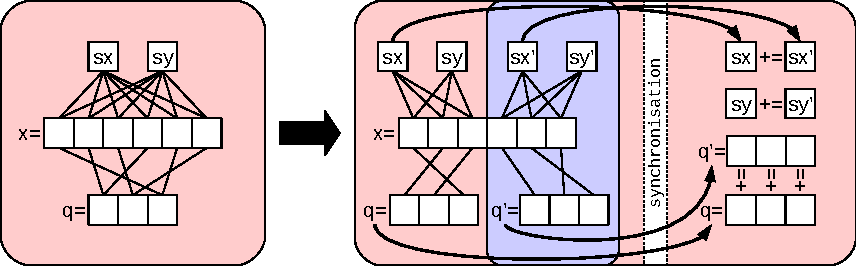
\includegraphics[width=0.99\textwidth]{figures/parallelisereduction.pdf}
\caption{Parallelisation of \Cref{complex-reduction-figure}:
         The input array \texttt{x} is split over two threads (red/blue)
         that operate on private copies of \texttt{sx}, \texttt{sy}, \texttt{q[]}.
         These copies are then merged after synchronisation.\parfillskip=0pt}
\label{nice-picture}
\end{figure}


\begin{figure}[p]
\centering
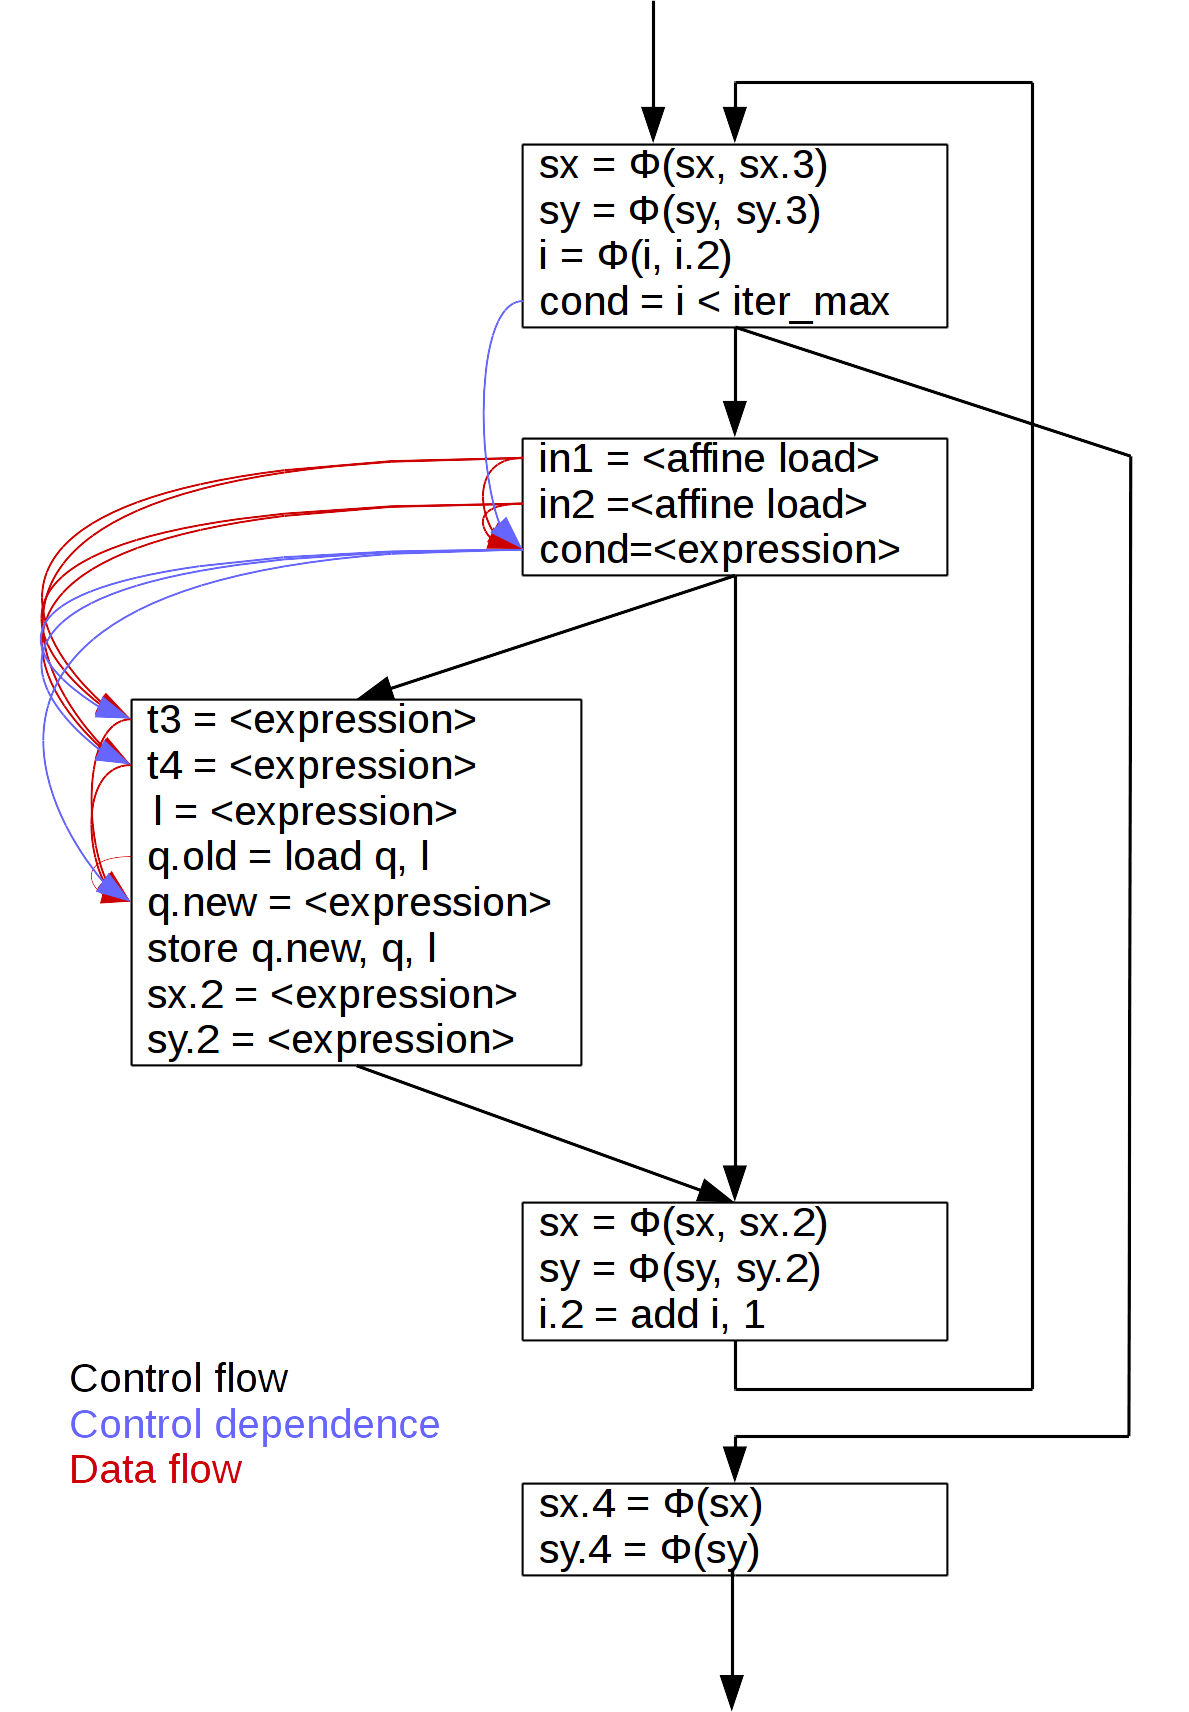
\includegraphics[width=\textwidth]{figures/nicepicture2.png}
\caption{A subset of the Data Flow, Control Flow and Control Dependences of
         \Cref{complex-reduction-figure}}
\label{nice-picture2}
\end{figure}

    \Cref{nice-picture2} gives an insight into why existing schemes do not
    detect such reductions by showing the compiler representation of this 
    program.
    The histogram update occurs in the 3rd basic block with the load, assign and
    store operations but it is by no means obvious that it is a safe reduction.
    In fact, accurately detecting reductions is non-trivial.
    If in the original program, shown in \Cref{complex-reduction-figure}, the
    condition on line 5 was changed to {\tt t1<=sx}, there would be no longer a
    legal reduction as there is now a control dependence on an intermediate
    result.
    This is turn would manifest as an additional data dependence edge from
    block 3 to block 2 in \Cref{nice-picture2}.
    Furthermore the code segment can only be classified as a reduction because
    all the function calls that are present are pure.
    Such details have to be checked to ensure correctness.
    What is needed is a way to specify these conditions exactly and to then
    automatically identify code regions that meet the constraints.

%% This becomes clearer when we write the operation with appropriately defined
%% types and using a custom overloaded operator as in Figure
%% \ref{complex-reduction-reformulated-figure}.

%% \begin{figure}[ht]
%% \begin{lstlisting}
%% for (i = 0; i < NK; i++) {
%%   Type2 value = {x[2*i], x[2*i+1]};
%%   result += value;
%% }
%% \end{lstlisting}
%% \begin{lstlisting}
%% struct Type1
%% {
%%   double q[10];
%%   double sx;
%%   double sy;
%% };

%% struct Type2
%% {
%%   double x1;
%%   double x2;
%% };

%% Type1& operator+=(Type1& a, const Type2& b) {
%%   double x1 = 2.0 * b.x1 - 1.0;
%%   double x2 = 2.0 * b.x2 - 1.0;
%%   double t1 = x1 * x1 + x2 * x2;

%%   if (t1 <= 1.0) {
%%     double t2 = sqrt(-2.0 * log(t1) / t1);
%%     double t3 = (x1 * t2);
%%     double t4 = (x2 * t2);
%%     int    l  = MAX(fabs(t3), fabs(t4));
%%     a.q[l]    = q[l] + 1.0;
%%     a.sx      = a.sx + t3;
%%     a.sy      = a.sy + t4;
%%   }
%%   return a;
%% }
%% \end{lstlisting}
%% \caption{Complex Reduction Reformulated}
%% \label{complex-reduction-reformulated-figure}
%% \end{figure}

%% The parallelisation strategy that is used for simple scalar reductions as
%% described above can not be applied directly here.
%% This is because it relies on the combining operator to be assciative.
%% As the operator that is defined in Figure
%% \ref{complex-reduction-reformulated-figure} is external (i.e.\ it operates on
%% two operands of different types), it clearly can not be associative in the
%% classical sense.

%% This associativity requirement can however be relaxed and we can introduce a
%% second operator $*=$ to complement $+=$ as in Figure
%% \ref{complement-operator-figure}.
%% Using these two operators we can proceed as with the simple sum example by
%% generating partial results in parallel with $+=$ and then merging them in the
%% end using $*=$.

%% \begin{figure}[ht]
%% \begin{lstlisting}
%% Type1& operator*=(Type1& a, const Type1& b) {
%%   for(int i = 0; i < 10; i++) a.q[i] += b.q[i];
%%   a.sx += b.sx; a.sy += b.sy;
%%   return a;
%% }
%% \end{lstlisting}
%% \caption{Complementary Reduction Operator}
%% \label{complement-operator-figure}
%% \end{figure}

%% In this complex reduction example we can see that the operation is fundamentally
%% composed of two elementary reduction operations.
%% The values of {\tt sx} and {\tt sy} are computed via scalar reductions and the
%% values of the array {\tt q} are computed via a histogram type computation.
%% These two building blocks span a large set of reduction operations that are
%% prevalent in many benchmark applications.

%% The definition of the $+=$ operator can be attained by applying strainghtforward
%% code transformations on the original source code.
%% The $*=$ operator can not be this easily deduced but is not dependent on he whole
%% operation performed in the $+=$ operator.

\section{Approach}

    There are three fundamental issues to address in exploiting reductions:
    detection, replacement and profitability.
    This chapter focuses on the reliable detection of reductions.
    For evaluation purposes, a preliminary code generation phase that generates
    parallel pthread code was also implemented.
    Profitability heuristics are important in practice to determine whether or
    not to apply parallelising code transformations.
    A simple profile-based approach was used for this work to determine whether
    or not to apply our optimisation.

%    Our method for the detection of reduction operations is based on a novel
%    constraint based description language for computational idioms and a generic
%    solver algorithm that searches in single static assignment compiler IR code
%    for subsets that satisfy them.
%    This decoupling of specification and detection enables us to build an
%    extensible system that can process complex reductions beyond the
%    capabilities of established approaches.

    In the next sub-sections, the constraint based specification approach with
    CAnDL is first motivated and described.
    The reduction idiom is then specified in this system and the CAnDL context
    is given.
    This is followed by a brief outline of how this is integrated in the
    LLVM compiler infrastructure.
    Finally, in the following section, an overview of the parallel code
    generation approach is given.

\subsection{Constraint based formulation}

    The motivation section described how reductions can be parallelised and
    suggested that the same basic technique can be applied to a wide range of
    generalised reductions.
    To enable compilers to exploit this, a precise definition of the kinds
    of computations that fit this approach is needed.
    This section formulates scalar and generalized reductions with constraints.

\subsubsection{Scalar Reductions}

    Informally, the following conditions are required to hold in a piece of
    source code for it to contain a computation that can be parallelised like a
    scalar reduction:
    \begin{enumerate}
        \item The code is contained in a for loop and the iteration space of the
              loop is known in advance (not necessarily at compile time).
        \item There is a scalar value $x$ that is updated in every iteration.
        \item One or multiple values $a_1,\dots,a_n$ are read from arrays and
              the indices are affine in the loop iterator.
        \item The updated value $x'$ is computed as a term only of $x$, the
              array values $a_1,\dots,a_n$ and values that are constant within
              the loop.
    \end{enumerate}

    The definition is broader than usual.
    In particular, it allows the reduction to encompass multiple input arrays.
    Furthermore, complex computations inside the reduction are possible, not
    just a scalar binary operator.
    Note that condition 2 is enforced only at SSA level.
    Finally, this definition does not yet contain a commutativity condition that
    would be neccesarry to allow the parallelisation to work.
    Instead, it also captures intrinsically sequential scalar reductions.

    \paragraph*{Example}
    Both variables \texttt{sx} and \texttt{sy} in
    \Cref{complex-reduction-figure} satisfy the conditions:
    Firstly, the iteration space of the loop is bounded by \texttt{NK}, which is
    constant.
    Secondly, within the SSA representation, both \texttt{sx} and \texttt{sy}
    are unconditionally updated via $\Phi$-instructions, shown previously in
    \Cref{nice-picture2}.
    This is despite the conditional statement in the original C representation
    of the program.
    Thirdly, exactly two values are read from the single input array \texttt{x}
    in every iteration, and the indices \texttt{2*i} and \texttt{2*i+1} are
    affine in \texttt{i}.
    Finally, the updated values depend only on the respective old values,
    the two values read from \texttt{x} and the constants \texttt{1.0} and
    \texttt{2.0}.
    This is due to the fact that all functions used in the computation are pure
    functions.

\begin{figure}[t]
\begin{lstlisting}[language=MyCpp]
sum = 0;
for(i = 0; i < n && sum < 10; i++)
    sum += a[i];
\end{lstlisting}
\begin{lstlisting}[language=MyCpp]
sum = 0;
for(i = 0; i < n; i++)
    b[i] += a[i];
\end{lstlisting}
\begin{lstlisting}[language=MyCpp]
chase = 0;
for(i = 0; i < n; i++)
    chase = a[chase];
\end{lstlisting}
\begin{lstlisting}[language=MyCpp,label={counterexamples},caption=
   {Counterexamples to the four conditions: None of these computations can be
    parallelised as scalar reductions.
    The first and last example implement the same program.\parfillskip=0pt}]
sum = 0;
active = false;
for(i = 0; i < n; i++) {
    sum += active?a[i]:0;
    active = active && (sum < 10);
}
\end{lstlisting}
\end{figure}

    \paragraph*{Counterexamles}
    \Cref{counterexamples} shows counterexamples to the four conditions,
    demonstrating why they are all needed in order to parallelise a given
    computation as a scalar reduction.

    In the first example, the iteration space is not known in advance, as the
    computation can be terminated depending on the input data.
    This makes it impossible to compute partial sums in parallel.
    The second example is straightforward, as there is no reduction variable
    that could be privatised.
    The loop could still be computed in parallel -- but not as a scalar
    reduction.
    The third example uses index calculations that are not affine in \texttt{i}.
    This prevents a straightforward distribution of the input array across
    threads.
    In this particular case, the index calculation also involves values other
    than \texttt{i}, preventing the computation of partial results entirely.
    The final example is equivalent to the first first, but breaks the fourth
    condition instead of the first.

\subsubsection{Generalized reductions or histograms}

    Histogram reductions are defined in the context of this work very similiarly
    to the previous definition of scalar reductions, with only some additional
    conditions:
    \begin{enumerate}
        \item The code is contained in a for loop and the iteration space of the
              loop is known in advance (not necessarily at compile time).
        \item One or multiple values $a_1,\dots,a_n$ are read from arrays and
              the indices are affine in the loop iterator.
        \item A value {\tt idx} is computed as a term only of the array values
              $a_1,\dots,a_n$ and values that are constant within the loop.
        \item A value $x$ is read from an array at index {\tt idx} and a
              modified value $x'$ is written at the same index.
              The writing might be control dependent only on $a_1,\dots,a_n$ and
              it may not be in a nested loop.
        \item The updated value $x'$ is computed as a term only of $x$, the
              array values $a_1,\dots,a_n$ and values that are constant within
              the loop.
    \end{enumerate}

    Again, additional commutativity conditions are required in order to restrict
    this to only parallelisable histograms.
    Note that the statement on control dependency and nested loops has to be
    made only for the write location, as writing to memory is the only side
    effect of the loop.

    \paragraph*{Example}
    The first two conditions are the same as those in the previous discussion of
    scalar reductions and were shown to hold for the loop in
    \Cref{complex-reduction-figure}.
    The array \texttt{q[]} also satisfies the remaining conditions:
    Firstly, the variable \texttt{l} corresponds to the value \texttt{idx}.
    Secondly, the element \texttt{q[l]} is read, modified and written.
    Lastly, the updated value is computed in a legal way, as it is obtained by
    merely adding a constant \texttt{1.0} to the previous value.

    \paragraph*{Counterexamples}
    Again, counterexamples are given in \Cref{counterexamples2} to give an
    intuition about the significance of conditions 3-5.

    In the first example, the index of the histogram is not computed from an
    input aray, but instead read from an input stream.
    This makes parallelisation as a histogram impossible, as the stream is only
    avaliable sequentially.
    In the second and third example, the computation is effectively stopped as
    soon as an index beyond a certain size occurs.
    Again, this can only be detected by sequentially going through the array,
    and therefore a parallel computation of partial results is not efficiently
    possible.
    This behaviour is demonstrated in two ways, by breaking conditions 4 and 5
    respectively.
    This shows the need to restrict both data flow and control flow of the
    histogram kernel.

\begin{figure}[t]
\lstset{basicstyle=\linespread{0.91}\ttfamily}
\begin{lstlisting}[language=MyCpp]
for(i = 0; i < n; i++)
    hist[getchar()] += 1;
\end{lstlisting}
\begin{lstlisting}[language=MyCpp]
active = true;
for(i = 0; i < n; i++) {
    if(a[i] > 9)
        active = false;
    if(active)
        hist[a[i]] += 1;
}
\end{lstlisting}
\begin{lstlisting}[language=MyCpp,label={counterexamples2},caption=
   {Counterexamples to the last three conditions:
    None of these computations can be parallelised as histograms.
    The final two example loops implement the same functionality.
    \parfillskip=0pt}]
active = 0;
for(i = 0; i < n; i++) {
    if(a[i] > 9)
        active = false;
    hist[a[i]] += active?1:0;
}
\end{lstlisting}
\end{figure}

\section{The Idiom Description Language}

\begin{table}[b]
    \lstset{keepspaces}
    \centering
    \begin{tabular}{|l|l|}
        \hline
        CAnDL & IDL\\
        \hline
        \hline
        {\lstinline[language=CAnDL]!∧!}, {\lstinline[language=CAnDL]!∨!} &
        {\lstinline[language=IDL]!and!}, {\lstinline[language=IDL]!or!} \\
        \hline
        {\lstinline[language=CAnDL]!include Spec({A}->{B}!}, &
        {\lstinline[language=IDL]!inherits Spec with {A} as {B}!}\\[-1mm]
        {\phantom{\lstinline[language=CAnDL]!include Spec(!}\lstinline[language=CAnDL]!{C}->{D})@{E}!} &
        {\phantom{\lstinline[language=IDL]!inherits Spec w!}\lstinline[language=IDL]!and {C} as {D} at {E}!}\\
        \hline
        {\lstinline[language=CAnDL]!{A}={B}!},
        {\lstinline[language=CAnDL]!{A}≠{B}!} &
        {\lstinline[language=IDL]!{A} is [not] equal to {B}!} \\
        \hline
        {\lstinline[language=CAnDL]!domination({A},{B})!} &
        {\lstinline[language=IDL]!{A} control flow dominates {B}!} \\
        \hline
        {\lstinline[language=CAnDL]!opcode{A} = store!} &
        {\lstinline[language=IDL]!{A} is store instruction!} \\
        \hline 
        {\lstinline[language=CAnDL]!{A} ∈ {B}.args!} &
        {\lstinline[language=IDL]!{A} has data flow to {B}!} \\
        \hline
    \end{tabular}
    \caption{The Idiom Description Language (IDL) is derived from CAnDL.
             However, it uses a more descriptive syntax, without uncommon
             unicode characters such as ``$\land$'', ``$\lor$'', ``$\in$'',
             and ``$\neq$''.\parfillskip=0pt}
    \label{CanDLtoIDL}
\end{table}

    For automatic detection during compilation, these conditions need to be
    specified formally in a constraint language.
    The CAnDL programming language from \Cref{chapter:candl} is taken as the
    basis for this formulation.
    However, additional language constructs are required in order to capture
    the kernel computations that are part of complex reduction and histogram
    computations.

    This extensions of CAnDL leads to the definition of the
    Idiom Description Language (IDL).
    IDL uses the solver infrastructure of CAnDL and retains the same high-level
    program structure.
    However, it extends the language and modifies the syntax to be more
    convenient for large-scale specifications by replacing uncommon Unicode
    characters.
    \Cref{CanDLtoIDL} shows syntax differences.

\subsection{Kernel Functions in IDL}

    Complex reduction and histogram computations can be expressed as a
    higher-order function.
    This means that the computational idiom is not just parameterised with
    numerical values, such as array dimensions, but contains kernel functions
    as parameters.
    To enable the capture of higher-order functions in IDL, additional
    constraint building blocks are required that go beyond what CAnDL
    provided.

    Specifically, IDL provides an additional atomic constraint based on
    generalised graph domination constraints, as previously described in
    \Cref{def:domconstr}, using the following syntax:
\begin{figure}[h]
    \centering
    \begin{tabular}{|c|}
        \hline
        $\textbf{all flow from }\text{\it variable\_tuple}\textbf{ or any origin to any of }\text{\it variable\_tuple}$\\
        $\textbf{ passes through at least one of }\text{\it variable\_tuple}$\\
        \hline
    \end{tabular}
\end{figure}

    \noindent
    The verbose syntax of this atomic constraint is quite discriptive, however
    some details require explanation.
    Firstly, ``flow'' in this constraint does not only capture data flow.
    To cover kernel functions with non-trivial control flow, the
    underlying graph on which this constraint operates is formed as an extension
    of the data flow graph $DFG_\mathcal F^*$.
    In addition to the data flow edges, it has an edge from each branch
    instruction to every instruction within all its targeted basic blocks.
    Secondly, as opposed to the control flow graph that is typically considered
    for dominance relationships, the resulting graph has no distinguished single
    ``origin''.
    Aside from the control entry, all non-pure function calls and all load
    operations are considered as origins of the graph.

    \Cref{kernelexample} demonstrates the significance of this definition.
    At the top is an SSA pseudocode representation of the complex reduction and
    histogram calculation from \Cref{complex-reduction-figure}, annotated in the
    right column with all the dependences described above.
    It is now possible to check the validity of the kernel function that is used
    within the loop for the reduction on \textit{sx} as follows:
    
\begin{figure}[h]
    \centering
    \begin{lstlisting}[language=IDL]
all flow from {loop_carried[1..3]} ([or]) any origin to any of
    {sx''} passes through ([at]) least one of
    {sx,t2,t5,precursor,backedge,ouside[0..N]}}
    \end{lstlisting}
\end{figure}

    \noindent
    This assumes that other constraints make sure that
    the ``\texttt{precursor}'' and ``\texttt{backedge}'' are determined and
    \texttt{outside[0..N]} contains
    all origins that lie outside the SESE region within which the kernel
    functions is considered.
    Furthermore, the array \texttt{loop\_carried} needs to be constrained to
    contain all loop-carried $\Phi$-instructions.

    Then it is easy to check that this constraint is satisfied:
    Control flow can only reach $sx''$ via the precursor in line 1 and the
    backedge in line 28.
    The other relevant graph origins for this example are only the load
    instructions in lines 6,9,18 and the additional $\Phi$-instructions.
    The three of these that can reach $sx''$ through the graph are explicitly
    killed as ``dominators''.

\begin{figure*}[p]
\centering
\begin{tabular}{|c|rl|l|}
\hline
\multicolumn{1}{|c}{\bf Block} &  \multicolumn{2}{|c|}{\bf Operation} & \multicolumn{1}{c|}{\bf Dependences} \\
\hline
\hline
\multirow{1}{*}{\bf loop}
  & {\bf 1:} & \textcolor{color_strings}{$\text{goto }loop$}&\textcolor{color_strings}{\bf outside the considered region}\\
\hline
\multirow{12}{*}{\bf loop}
  & {\bf  2:} & \textcolor{gray}{$i\leftarrow \Phi(entry:0,\ loop:i')$}&\textcolor{gray}{loop carried data flow}\\[-2mm]
  & {\bf  3:} & \textcolor{color_types}{$sx\leftarrow \Phi(entry:0.0,\ loop:sx'')$}&\textcolor{color_types}{\bf loop carried data flow}\\[-2mm]
  & {\bf  4:} & \textcolor{gray}{$sy\leftarrow \Phi(entry:0.0,\ loop:sy'')$}&\textcolor{gray}{loop carried data flow}\\[-2mm]
  & {\bf  5:} & \textcolor{gray}{$t_1\leftarrow 2\cdot i$}&\textcolor{gray}{control({\bf 1, 28}), data({\bf 2})}\\[-2mm]
  & {\bf  6:} & \textcolor{color_types}{$t_2\leftarrow\textbf{load }x[t_1]$}&\textcolor{color_types}{\bf origin of data flow}\\[-2mm]
  & {\bf  7:} & $t_3\leftarrow 2.0\cdot t_2-1.0$&{\bf control({\bf 1, 28}), data({\bf 6})}\\[-2mm]
  & {\bf  8:} & \textcolor{gray}{$t_4\leftarrow 2\cdot i+1$}&\textcolor{gray}{control({\bf 1, 28}), data({\bf 2})}\\[-2mm]
  & {\bf  9:} & \textcolor{color_types}{$t_5\leftarrow\textbf{load }x[t_4]$}&\textcolor{color_types}{\bf origin of data flow}\\[-2mm]
  & {\bf 10:} & $t_6\leftarrow 2.0\cdot t_5-1.0$&{\bf control({\bf 1, 28}), data({\bf 9})}\\[-2mm]
  & {\bf 11:} & $t_7\leftarrow t_3\cdot t_3+t_6\cdot t_6$&{\bf control({\bf 1, 28}), data({\bf 7, 10})}\\[-2mm]
  & {\bf 12:} & $t_8\leftarrow t_7\leq1.0$&{\bf control({\bf 1, 28}), data({\bf 11})}\\[-2mm]
  & {\bf 13:} & $\text{if }t_8\text{ goto }ifblock\text{ else }uncond$&{\bf control({\bf 1, 28}), data({\bf 12})}\\
\hline
\multirow{10}{*}{\bf ifblock}
 & {\bf 14:} & $t_9\leftarrow sqrt(-2.0\cdot log(t_7) / t_7)$&{\bf control({\bf 13}), data({\bf 11})}\\[-2mm]
 & {\bf 15:} & $t_{10}\leftarrow t_3*t_9$&{\bf control({\bf 13}), data({\bf 7, 14})}\\[-2mm]
 & {\bf 16:} & \textcolor{gray}{$t_{11}\leftarrow t_6\cdot t_9$}&\textcolor{gray}{control({\bf 13}), data({\bf 10, 14})}\\[-2mm]
 & {\bf 17:} & \textcolor{gray}{$l\leftarrow MAX(fabs(t_{10}), fabs(t_{11}))$}&\textcolor{gray}{control({\bf 13}), data({\bf 15, 16})}\\[-2mm]
 & {\bf 18:} & \textcolor{gray}{$t_{12}\leftarrow\textbf{load }q[l]$}&\textcolor{gray}{origin of data flow}\\[-2mm]
 & {\bf 19:} & \textcolor{gray}{$t_{13}\leftarrow t_{12}+1$}&\textcolor{gray}{control({\bf 13}), data({\bf 18})}\\[-2mm]
 & {\bf 20:} & \textcolor{gray}{$\textbf{store }q[l]\leftarrow t_{13}$}&\textcolor{gray}{control({\bf 13}), data({\bf 19})}\\[-2mm]
 & {\bf 21:} & $sx'\leftarrow sx+t_{10}$&{\bf control({\bf 13}), data({\bf 3, 15})}\\[-2mm]
 & {\bf 22:} & \textcolor{gray}{$sy'\leftarrow sy+t_{11}$}&\textcolor{gray}{control({\bf 13}), data({\bf 4, 16})}\\[-2mm]
 & {\bf 23:} & $\text{goto }uncond$&{\bf control({\bf 13})}\\
\hline
\multirow{5}{*}{\bf uncond}
 & {\bf 24:} & \textcolor{color_keywords}{$sx''\leftarrow\Phi(loop:sx,\ ifblock:sx')$}&\textcolor{color_keywords}{\bf control({\bf 13, 23}), data({\bf 3, 21})}\\[-2mm]
 & {\bf 25:} & \textcolor{gray}{$sy''\leftarrow\Phi(loop:sy,\ ifblock:sy')$}&\textcolor{gray}{control({\bf 13, 23}), data({\bf 4, 22})}\\[-2mm]
 & {\bf 26:} & \textcolor{gray}{$i'\leftarrow i+1$}&\textcolor{gray}{control({\bf 13, 23}), data({\bf 2})}\\[-2mm]
 & {\bf 27:} & \textcolor{gray}{$t_{14}\leftarrow i' < NK$}&\textcolor{gray}{control({\bf 13, 23}), data({\bf 26})}\\[-2mm]
 & {\bf 28:} & \textcolor{color_strings}{$\text{if }t_{14}\text{ goto }loop\text{ else }exit$}&\textcolor{color_strings}{\bf outside the considered region}\\
\hline
\end{tabular}

\begin{tabular}{|cl|}
\multicolumn{2}{c}{{\bf function} kernel($sx, t_2, t_5$)}\\
\hline
\multirow{5}{*}{\bf entry} & $t_3 \leftarrow 2.0\cdot t_2-1.0$\\[-2mm]
                           & $t_6 \leftarrow 2.0\cdot t_5-1.0$\\[-2mm]
                           & $t_7 \leftarrow t_3\cdot t_3+t_6\cdot t_6$\\[-2mm]
                           & $t_8 \leftarrow t_7\leq 1.0$\\[-2mm]
                           & $\text{if }t_8\text{ goto }ifblock\text{ else }uncond$\\
\hline
\multirow{4}{*}{\bf ifblock} & $t_9\leftarrow sqrt(-2.0\cdot log(t_7) / t_7)$\\[-2mm]
                             & $t_{10}\leftarrow t_3\cdot t_9$\\[-2mm]
                             & $sx'\leftarrow sx+t_{10}$\\[-2mm]
                             & $\text{goto }uncond$\\
\hline
\multirow{2}{*}{\bf uncond} & $sx''\leftarrow\Phi(loop:sx,\ ifblock:sx')$\\[-2mm]
                            & $\text{return }sx''$\\
\hline
\end{tabular}
\caption{A kernel function is identified within the SSA pseudocode at the top
    (cf.\ \Cref{complex-reduction-figure}):
    The value of $sx''$ is calculated in the SESE region spanning lines 2--27
    as a pure function of only \mbox{$sx$, $t_2$, and $t_5$}.
    This is determined by starting from $sx''$
    (\textcolor{color_keywords}{\bf blue}) and following the dependences on the
    right, checking that all paths end in the predetermined function arguments
    \mbox{$sx$, $t_1$ and $t_5$ (\textcolor{color_types}{\bf red})}.
    The kernel function can then be extracted and valid SSA
    reconstructed, as shown at the bottom.
    \parfillskip=0pt}
\label{kernelexample}
\end{figure*}

%    Kernel functions are sections of code that are side-effect free and
%    can be separated out. Identifying side-effect free code is useful in
%    many types of compiler optimisation.  It can be expressed in CAnDL, as
%    shown in \Cref{fig:kernel}.
%
%\begin{figure}[ht]
%\begin{lstlisting}[language=CAnDL,label={fig:kernel},caption=
%   {CAnDL Formulation of Kernel Functions}]
%Constraint KernelFunction
%( collect i N
%∧ ( include LocalConst({outer}->{begin}*@*{closure[i]}
%  ∧ ir_type{closure[i].value} != literal
%  ∧ {closure[i].use} ([$\tt \in$]) {closure[i].value}.args
%  ∧ domination({inner}, {closure[i].use}))
%∧ collect i N data_origin{tainted1[i]}
%∧ collect i N
%∧ ( domination({outer}, {tainted2[i]})
%  ∧ strict_domination({tainted2[i]}, {inner}))
%∧ calculated_from(
%   {tainted1[0..N],tainted2[0..N]},
%   {origin[0..N],closure[0..N].value,input[0..N]},
%   {output}))
%End
%\end{lstlisting}
%\end{figure}
%
%    Essentially, this set of contraints captures the computation of a
%    single \texttt{output} value from a set of specified \texttt{input}
%    values as well as a set of automatically captured \texttt{closure}
%    variables.  The computation for \texttt{output} should be such that it
%    can be replaced with a function call that is free of side effects and
%    takes only the \texttt{input} and \texttt{closure} variables as
%    arguments.
%
%    In addition to these variables, there are two non-obvious additional
%    variables involved: \texttt{outer} and \texttt{inner}.
%    These set boundaries in the control flow as follows: Closure values have to
%    be computed before \texttt{outer} and the computation that results in outer
%    is performed after \texttt{inner}.
%    Usually these will be derived from loops nests, where \texttt{outer} is the
%    entry to the outermost loop and \texttt{inner} is the entry to the innermost
%    loop.
%    The actual core constraint is then a generalized dominance relationship in
%    the program dependence graph.
%
%    The use of the sets \texttt{tainted1} and \texttt{tainted2} makes sure that
%    no impure functions are used in computing \texttt{output} and the entire
%    computation is performed after \texttt{inner} (ruling out e.g.\ loop carried
%    variabls from outer loops).
%

\subsection{Complex Reductions and Histograms in IDL}

    These definitions need be formulated precisely in a constraint language in a
    form that can automatically verified by a constraint solver.
    So we  developed a formal language  to achieve this.

\begin{figure*}[p]
\begin{lstlisting}[language=IDL,label={IDLcomplexred},caption=
   {Complex reductions and histograms as an IDL specification}]
Constraint ComplexReduction
( inherits For and
  collect k 32
  ( inherits VectorRead
        with {iterator} as {idx}
         and {read_value[k]} as {value}
         and {loop.begin} as {begin}
                          at {read[k]}) and
  collect k 2
  ( inherits HistoPart
        with {begin} as {begin}
         and {read}  as {read}
         and {loop}  as {loop}
         and {read_value} as {read_value}
                          at {histo[k]}) and
  collect k 2
  ( inherits ScalarPart
        with {begin}      as {begin}
         and {iterator}   as {iterator}
         and {loop}       as {loop}
         and {read_value} as {read_value}
          at {scalar[k]}) and
  {scalar[0].kernel.output} is not the same ([as])
      {histo[0].update.store_instr} and
  collect i 2
  ( {histo[i].update.store_instr} is store instruction and
    {loop.begin} control flow dominates
        {histo[i].update.store_instr} and
    {loop.end} control flow post dominates
        {histo[i].update.store_instr}) and
  collect i 32
  ( inherits LocalFunctionCall
        with {begin} as {begin}
         and {loop.end} as {end} at {call[i]}) and
  collect i 32
  ( inherits LocalFunctionCall
        with {begin} as {begin}
         and {loop.end} as {end} at {call[i]} and
    {call[i].function} has attribute pure))
End
\end{lstlisting}
\end{figure*}

\Cref{for-loop-constraints} shows
the formulation of the first condition regarding the type of loop structure allowed in this language.  
\Cref{dom-expr-constraints} specifies the fourth condition.
The first item in \Cref{dom-expr-constraints}  requires some clarifications.
When we say that a node $a$ is {\tt 1+dominat}ed by nodes $b_1,\dots,b_n$, we do not mean that each individual node $b_k$ dominates $a$.
Instead we mean that each path from a source (non pure function call, load instruction) to $a$ has to pass through {\em at least one} of the nodes $b_1,\dots,b_n$.
This ensures that no other inputs influence the value of $x'$.
We use the program dependence graph instead of the data flow graph to also allow well behaved control flow.
It is obtained as the union of data flow and control dependence graph.
This is the reason that we have to include \texttt{loop jump}, which reaches $x'$ in the program dependence graph.
Including it takes care of the control flow outside of the loop body.

The other conditions, and therefore the whole reduction idiom, can be specified using the same basic constraints as well.
Due to space we omit further details.

\newpage

\section{Code Generation}
%% To give speedup results in the evaluation section we implemented some functionality to use our detection functionality.
%% More precisely we implemented a code transformation pass that automatically parallelizes histogram reductions.
%% We did not implement equivalent functionality for scalar reductions as preliminary runtime coverage results showed them to be almost irrelevant for the performance of many benchmark programs.

    The code generation pass immediately follows the CAnDL-generated detection
    pass.
    It uses the detected constraint solution and parallelises the corresponding
    loops.
    For each reduction that is found, all the relevant input arrays and scope
    variables are taken from the solution and packed into a structure together
    with potential histogram arrays and some additional parameters.
    A function is generated that takes this structure as its only parameter.
    Depending on the amount of processors in the system and the recursion
    depth, the function decides whether to bisect its workload recursively.
    If not, it simply executes the histogram functionality.
    Otherwise it uses \texttt{pthread\_create} to offload half of its
    workload into another thread.
    For this, it copies its parameter array but replaces the histogram array
    with a newly allocated copy.
    After both threads finished their work, the copy is merged with the original
    histogram element wise and the copy is deallocated.

    In general, the size of the histogram array can not be determined at
    compile time.
    We therefore use dynamic boundary checking in all the branched off threads
    and reallocate the histogram array when necessary.
    This introduces some overhead but proved acceptable in many benchmark
    programs.

    Optimal code generation was not the main focus of this research and more
    sophisticated methods for the parallelization of reductions could be added.

\section{Experimental Setup}

\subsection{Benchmarks}

    The prototype idiom detection pass pass applied to C versions of the
    NAS Parallel Benchmarks.
    Specifically, the SNU NPB implementation by the Seoul National University
    was used, which contains the original 8 NAS benchmarks plus two of the newer
    unstructured components UA and DC.

    The approach was also evaluated on all Parboil and Rodinia benchmark
    programs.
    This constitutes 40 programs in total of varying length.
    EP in NPB for instance is a single file of 324 lines in length.
    Leukocyte in Rodinia by contrast contains over 50 files.
    For each of the individual benchmark programs, the number of distinct scalar
    and histogram reductions found was collected.

\subsection{Alternative approaches}

    To provide a useful comparison we evaluated against two competitive
    existing approaches. The first is a  recently published approach that
    detects reductions within the polyhedral framework, the second is a mature
    state-of-the-art industrial compiler.

\paragraph*{Polly-Reduction}

    \citet{Doerfert2015Polly} developed a compiler analysis and transformation
    within Polly that detects reductions in Static Control Parts of programs.
    This is implemented in Polly, an LLVM based polyhedral compiler.
    The polyhedral model is extremely powerful when applicable and as Polly is
    also LLVM based, this allows for a comparison against another approach that
    uses the same IR and compiler infrastructure.

    The sequential versions of the benchmark programs were compiled using
    version 3.9 of the Clang compiler with Polly built in.
    The SCoPs that Polly detected with the compiler options \texttt{-O3
    -mllvm -polly -mllvm -polly-export} were gathered during compilation.
    As any Polly based approach only works within these SCoPs, this gives an
    upper bound for the Polly-Reduction method.
    Reductions within the SCoPS were then manually identified, and any reduction
    within a SCoP was counted as a hit for Polly-Reduction.
    This gives an optimistic estimate as to what coverage a polyhedral based
    approach to reduction operations, such as the one presented in
    \citet{Doerfert2015Polly}, can achieve.

\paragraph*{Intel icc}

    The Intel icc compiler is a mature compiler incorporating
    auto-parallelization and vectorization.
    It uses simpler data dependence analysis rather than the polyhedral model as
    its fundamental analysis tool.
    It is therefore less powerful than polyhedral approaches, but sometimes more
    robust in practice.

    For this evaluation, the benchmarks were compiled with the
    \texttt{-parallel -qopt-report} options.
    This generated icc optimisation reports.
    Intel icc does not explicitly report reductions, but any reduction that was
    within a loop that icc considered to be parallelisable was counted.
    This also included in the detection results all those loops that icc
    considered possible but inefficient.


\subsection{Platform}

    To determine runtime coverage and performance, the benchmarks were evaluated
    on a 64 core machine with four AMD Opteron(tm) 6376 processors and one
    terrabyte of RAM.

%{\em MOB put in more details on platform}


%% To measure the runtime coverage of the detected reductions we then used standard profiling techniques to weed out
%% reductions located in functions that are irrelevant to the runtime.
%% For the remaining reduction we annotated the source code with timing routines to investigate individual runtime
%% impact.
%% This of course modified the original program but the results were quite clear-cut and so we did not worry about this.

%% For comparison we also evaluated the NAS Parallel Benchmarks using Polly and the Intel icc compiler.

\section{Results}

This section first presents the number of reduction found by the
various schemes. This is followed an analysis of how significant each
reduction is. Finally we show the performance impact of our scheme.
   
\subsection{Discovery}
We applied our approach to the three benchmark suites  and the results are shown in \Cref{npb_spotted,parboil_spotted,rodinia_spotted}. 
Across the suites, our detection algorithms
was able to identify 84 scalar reductions and 6 histogram reductions.

%{\em MOB Why no reductions in FT and LU}.
There were reductions detected in nearly all of the individual NAS benchmarks with UA having the highest number, 11.
Reductions were less prevalent in Parboil with 5 out of 11
benchmarks having reductions. Cutcp had the most, 7, reductions. 
%{\em MOB Why no reductions in spmv,stencil}.
Surprisingly, the Rodinia benchmark collection contained many more identifiable reductions than Parboil.
Our program detected reductions in 15 out of the 19 benchmarks, with 9 reductions in the particlefilter program alone.

There were some regions that we were able to identify as reductions manually that our system did not find.
This was generally the case when the reduction loop was not the innermost loop, e.g.\ in the following code segment from SP.
\begin{lstlisting}[language=MyCpp]
for (k = 1; k <= nz2; k++) {
  for (j = 1; j <= ny2; j++) {
    for (i = 1; i <= nx2; i++) {
      for (m = 0; m < 5; m++) {
        add = rhs[k][j][i][m];
        rms[m] = rms[m] + add*add;
      } 
    } 
  } 
}
\end{lstlisting}


Histogram reductions are rarer than scalar reductions.  However
our algorithm was able to detect 3 in NAS, 2 in Parboil and 1 in
Rodinia.   They were still fundamentally sums but contained
complex expressions to compute the update values.  An  example is the
inner most loop of this code snippet from backprop.
\begin{lstlisting}[language=MyCpp]
for (j = 1; j <= nh; j++) {
  h = hidden[j];
  sum = 0.0;
  for (k = 1; k <= no; k++) {
    sum += delta_o[k] * who[j][k];
  }
  delta_h[j] = h * (1.0 - h) * sum;
  errsum += ABS(delta_h[j]);
}
\end{lstlisting}
%{\em MOB say something interesting about the reductions found. Any unusual ones}

%% The spotted hsitogram reductions looked much more diverse than the scalar reductions, which were mostly still slightly generalised sums of floating point numbers.
%% We already saw the reduction in EP in figure \ref{complex-reduction-figure}.
One interesting examples is tpacf from the Parboil benchmarks.
In this reduction, the histogram index is computed via a binary search in an additional array.
On the other hand the performance bottleneck of IS is a plain histogram without any complications.
\begin{lstlisting}[language=MyCpp]
for( i=0; i<NUM_KEYS; i++ )
  key_buff_ptr[key_buff_ptr2[i]]++;
\end{lstlisting}
%{\em MOB say something interesting about the histograms found. Any unusual ones}

Polly+Reductions, however, is able to find just 2 scalar reductions in
the NAS benchmarks: BT and SP, 1 in Parboil: sgemm and 1 in
Rodina:leukocte. 4 in total compared to the 84 found by our scheme. It
was unable to detect any of the histogram reductions.

In contrast, the Intel icc compiler was more successful than Polly in detecting 
reductions: 25  out if 38 in NAS, 3 out of 11 in Parboil and 23 out of 38 in Rodinia.
Unfortunately, these were all scalar reductions; no histograms were detected.

%% Only one of the histogram reduction operations need a slight
%% relaxation of our constraint system (tpacf from the Parboil
%% benchmarks).  The figures \ref{npb_spotted}, \ref{parboil_spotted}
%% and \ref{rodinia_spotted} show the detection results in detail.

\pgfplotstableread[row sep=\\,col sep=&]{
benchmark & scalar reductions & histogram reductions & total reductions\\
BT &  2 & 0 &  2 \\
CG &  8 & 1 &  9\\
DC &  6 & 0 &  6\\
EP &  3 & 1 &  4\\
FT &  0 & 0 &  0\\
IS &  4 & 1 &  5\\
LU &  0 & 0 &  0\\
MG &  1 & 0 &  1\\
SP &  2 & 0 &  2\\
UA & 11 & 0 & 11\\
}\NASDetectionData

\pgfplotstableread[row sep=\\,col sep=&]{
benchmark & scalar reductions & histogram reductions & total reductions\\
bfs          & 0 & 0 & 0\\
cutcp        & 7 & 0 & 7\\
histo        & 0 & 1 & 1\\
lbm          & 0 & 0 & 0\\
mri-gridding & 0 & 0 & 0\\
mri-q        & 0 & 0 & 0\\
sad          & 1 & 0 & 1\\
sgemm        & 1 & 0 & 1\\
spmv         & 0 & 0 & 0\\
stencil      & 0 & 0 & 0\\
tpacf        & 0 & 1 & 1\\
}\ParboilDetectionData

\pgfplotstableread[row sep=\\,col sep=&]{
benchmark & scalar reductions & histogram reductions & total reductions\\
backprop       & 2 & 0 & 2\\
bfs            & 0 & 0 & 0\\
b+tree         & 2 & 0 & 2\\
cfd            & 0 & 0 & 0\\
heartwall      & 3 & 0 & 3\\
hotspot        & 1 & 0 & 1\\
hotspot3D      & 2 & 0 & 2\\
kmeans         & 4 & 1 & 5\\
lavaMD         & 1 & 0 & 1\\
leukocyte      & 2 & 0 & 2\\
lud            & 3 & 0 & 3\\
mummergpu      & 1 & 0 & 1\\
myocyte        & 2 & 0 & 2\\
nn             & 1 & 0 & 1\\
nw             & 0 & 0 & 0\\
particlefilter & 9 & 0 & 9\\
pathfinder     & 0 & 0 & 0\\
srad           & 2 & 0 & 2\\
streamcluster  & 3 & 0 & 3\\
}\RodiniaDetectionData

\pgfplotstableread[row sep=\\,col sep=&]{
benchmark & scalar reductions & histogram reductions\\
BT & 0 & 0\\
CG & 0.0150372131 & 0\\
DC & 0 & 0\\
EP & 0 & 0.46702\\
FT & 0 & 0\\
IS & 0 & 0.9837540635\\
LU & 0 & 0\\
MG & 0 & 0\\
SP & 0 & 0\\
UA & 0.0773052818 & 0\\
}\NASCoverageData

\pgfplotstableread[row sep=\\,col sep=&]{
benchmark & scalar reductions & histogram reductions\\
bfs          & 0 & 0\\
cutcp        & 0 & 0\\
histo        & 0 & 0.9423193647\\
lbm          & 0 & 0\\
mri-gridding & 0 & 0\\
mri-q        & 0 & 0\\
sad          & 0 & 0\\
sgemm        & 0.9780887552 & 0\\
spmv         & 0 & 0\\
stencil      & 0 & 0\\
tpacf        & 0 & 0.999213841\\
}\ParboilCoverageData


\pgfplotstableread[row sep=\\,col sep=&]{
benchmark & histogram reductions\\
backprop       & 0\\
bfs            & 0\\
b+tree         & 0\\
cfd            & 0\\
heartwall      & 0\\
hotspot        & 0\\
hotspot3D      & 0\\
kmeans         & 0.9998935921\\
lavaMD         & 0\\
leukocyte      & 0\\
lud            & 0\\
mummergpu      & 0\\
myocyte        & 0\\
nn             & 0\\
nw             & 0\\
particlefilter & 0\\
pathfinder     & 0\\
srad           & 0\\
streamcluster  & 0\\
}\RodiniaCoverageData


\pgfplotstableread[row sep=\\,col sep=&]{
benchmark & reduction SCoPs & other SCoPs\\
BT &  1 & 8\\
CG &  0 & 1\\
DC &  0 & 0\\
EP &  0 & 0\\
FT &  0 & 1\\
IS &  0 & 0\\
LU &  0 & 5\\
MG &  0 & 5\\
SP &  1 & 17\\
UA &  0 & 0\\
    }\NASPollyData

\pgfplotstableread[row sep=\\,col sep=&]{
benchmark & reduction SCoPs & other SCoPs\\
bfs          & 0 & 0\\
cutcp        & 0 & 0\\
histo        & 0 & 0\\
lbm          & 0 & 2\\
mri-gridding & 0 & 0\\
mri-q        & 0 & 0\\
sad          & 0 & 1\\
sgemm        & 1 & 0\\
spmv         & 0 & 0\\
stencil      & 0 & 1\\
tpacf        & 0 & 0\\
}\ParboilPollyData

\pgfplotstableread[row sep=\\,col sep=&]{
benchmark & reduction SCoPs & other SCoPs & remainder SCoPs\\
backprop       & 0 & 2 & 0 \\
bfs            & 0 & 0 & 0 \\
b+tree         & 0 & 0 & 0 \\
cfd            & 0 & 5 & 0 \\
heartwall      & 0 & 1 & 0 \\
hotspot        & 0 & 0 & 0 \\
hotspot3D      & 0 & 0 & 0 \\
kmeans         & 0 & 2 & 0 \\
lavaMD         & 0 & 0 & 0 \\
leukocyte      & 0 & 2 & 0 \\
lud            & 1 & 1 & 0 \\
mummergpu      & 0 & 0 & 0 \\
myocyte        & 0 & 1 & 0 \\
nn             & 0 & 0 & 0 \\
nw             & 0 & 0 & 0 \\
particlefilter & 0 & 0 & 0 \\
pathfinder     & 0 & 0 & 0 \\
srad           & 0 & 0 & 0 \\
streamcluster  & 0 & 0 & 0 \\
}\RodiniaPollyData


\pgfplotstableread[row sep=\\,col sep=&]{
benchmark & detected by icc & not detected by icc\\
BT &  2 & 0\\
CG &  8 & 1\\
DC &  3 & 3\\
EP &  1 & 3\\
FT &  0 & 0\\
IS &  0 & 5\\
LU &  0 & 0\\
MG &  1 & 0\\
SP &  0 & 0\\
UA & 10 & 1\\
}\NASICCData

\pgfplotstableread[row sep=\\,col sep=&]{
benchmark & detected by icc & not detected by icc\\
bfs          & 0 & 0\\
cutcp        & 1 & 6\\
histo        & 0 & 1\\
lbm          & 0 & 0\\
mri-gridding & 0 & 0\\
mri-q        & 0 & 0\\
sad          & 1 & 0\\
sgemm        & 1 & 0\\
spmv         & 0 & 0\\
stencil      & 0 & 0\\
tpacf        & 0 & 1\\
}\ParboilICCData

\pgfplotstableread[row sep=\\,col sep=&]{
benchmark & detected by icc & not detected by icc\\
backprop       & 1 & 1\\
bfs            & 0 & 0\\
b+tree         & 0 & 2\\
cfd            & 0 & 0\\
heartwall      & 3 & 0\\
hotspot        & 0 & 1\\
hotspot3D      & 1 & 1\\
kmeans         & 2 & 3\\
lavaMD         & 0 & 1\\
leukocyte      & 0 & 2\\
lud            & 2 & 1\\
mummergpu      & 0 & 1\\
myocyte        & 2 & 0\\
nn             & 0 & 1\\
nw             & 0 & 0\\
particlefilter & 8 & 1\\
pathfinder     & 0 & 0\\
srad           & 2 & 0\\
streamcluster  & 2 & 1\\
}\RodiniaICCData

%% \begin{figure*}[p]
%%   \centering
%%   \begin{subfigure}[b]{0.49\textwidth}
%%     \centering
%%     \begin{tikzpicture}
%%       \begin{axis}[ybar=0.0, ymajorgrids, xtick style={transparent}, xtick=data,legend style={font=\small},
%%                    xticklabel pos=upper, bar width=.15cm,
%%                    ymin=0, ymax=13, ytick={0,2,4,6,8,10,12},
%%                    symbolic x coords={BT,CG,DC,EP,FT,IS,LU,MG,SP,UA},
%%                    xticklabel style={rotate=0},
%%                    width=9cm, height=5.56230589875cm, legend style={at={(3.5cm,3.88cm)},anchor=north}]
%%         \addplot [bar shift=-0.15cm,fill=black!80!white] table[x=benchmark,y=total reductions]{\NASDetectionData};
%%         \addplot [bar shift=-0.15cm,fill=lightgray!80!white] table[x=benchmark,y=scalar reductions]{\NASDetectionData};
%%         \addplot [bar shift=0.00cm,style={pattern=crosshatch dots}] table[x=benchmark,y=detected by icc]{\NASICCData};
%%         \addplot [bar shift=0.15cm,style={pattern=crosshatch}] table[x=benchmark,y=reduction SCoPs]{\NASPollyData};
%%         \legend{histogram reductions, scalar reductions,icc reductions, Polly+reductions}
%%       \end{axis}
%%     \end{tikzpicture}
%%     \caption{NAS Parallel Benchmarks}
%%     \label{npb_spotted}
%%   \end{subfigure}
%%   \begin{subfigure}[b]{0.49\textwidth}
%%     \centering
%%     \begin{tikzpicture}
%%       \begin{axis}[ybar=0.0, ymajorgrids, xtick style={transparent}, xtick=data,legend style={font=\small},
%%                    xticklabel pos=upper, bar width=.15cm,
%%                    ymin=0, ymax=9, ytick={0,2,4,6,8},
%%                    symbolic x coords={bfs,cutcp,histo,lbm,mri-gridding,mri-q,sad,sgemm,spmv,stencil,tpacf},
%%                    xticklabel style={rotate=90},
%%                    width=9cm, height=5.56230589875cm, legend pos=north east]
%% %        \addplot table[x=benchmark,y=scalar reductions]{\ParboilDetectionData};
%% %        \addplot table[x=benchmark,y=histogram reductions]{\ParboilDetectionData};
%% %        \legend{scalar reductions, histogram reductions}
%%         \addplot [bar shift=-0.15cm,fill=black!80!white] table[x=benchmark,y=total reductions]{\ParboilDetectionData};
%%         \addplot [bar shift=-0.15cm,fill=lightgray!80!white] table[x=benchmark,y=scalar reductions]{\ParboilDetectionData};
%%         \addplot [bar shift=0.00cm,style={pattern=crosshatch dots}] table[x=benchmark,y=detected by icc]{\ParboilICCData};
%%         \addplot [bar shift=0.15cm,style={pattern=crosshatch}] table[x=benchmark,y=reduction SCoPs]{\ParboilPollyData};
%%         \legend{histogram reductions, scalar reductions,icc reductions, Polly+reductions}
%%       \end{axis}
%%     \end{tikzpicture}
%%     \caption{Parboil Benchmarks}
%%     \label{parboil_spotted}
%%   \end{subfigure}
%%   \begin{subfigure}[b]{\textwidth}
%%     \centering
%%     \begin{tikzpicture}
%%       \begin{axis}[ybar=0.0, ymajorgrids, xtick style={transparent}, xtick=data,legend style={font=\small},
%%                    xticklabel pos=upper, bar width=.15cm,
%%                    ymin=0, ymax=11, ytick={0,2,4,6,8,10},
%%                    symbolic x coords={backprop,bfs,b+tree,cfd,heartwall,hotspot,hotspot3D,kmeans,lavaMD,leukocyte,lud,mummergpu,myocyte,nn,nw,particlefilter,pathfinder,srad,streamcluster},
%%                    xticklabel style={rotate=90},
%%                    width=14.5623058988cm, height=5.56230589875cm, legend pos=north west]
%% %        \addplot table[x=benchmark,y=scalar reductions]{\RodiniaDetectionData};
%% %        \addplot table[x=benchmark,y=histogram reductions]{\RodiniaDetectionData};
%% %        \legend{scalar reductions, histogram reductions}
%%         \addplot [bar shift=-0.15cm,fill=black!80!white] table[x=benchmark,y=total reductions]{\RodiniaDetectionData};
%%         \addplot [bar shift=-0.15cm,fill=lightgray!80!white] table[x=benchmark,y=scalar reductions]{\RodiniaDetectionData};
%%         \addplot [bar shift=0.00cm,style={pattern=crosshatch dots}] table[x=benchmark,y=detected by icc]{\RodiniaICCData};
%%         \addplot [bar shift=0.15cm,style={pattern=crosshatch}] table[x=benchmark,y=reduction SCoPs]{\RodiniaPollyData};
%%         \legend{histogram reductions, scalar reductions,icc reductions, Polly reductions}
%%       \end{axis}
%%     \end{tikzpicture}
%%     \caption{Rodinia}
%%     \label{rodinia_spotted}
%%   \end{subfigure}
%%   \caption{Spotted Reductions in the Individual Benchmark Collections}
%% \end{figure*}

\begin{figure}[ht]%{0.49\textwidth}
  \centering
%  \begin{subfigure}[b]
%    \centering
    \begin{tikzpicture}
      \begin{axis}[ybar=0.0, ymajorgrids, xtick style={transparent}, xtick=data,legend style={font=\small},
                   xticklabel pos=upper, bar width=.15cm,
                   ymin=0, ymax=13, ytick={0,2,4,6,8,10,12},
                   symbolic x coords={BT,CG,DC,EP,FT,IS,LU,MG,SP,UA},
                   xticklabel style={rotate=0},
                   width=9cm, height=5.56230589875cm, legend style={at={(3.5cm,3.88cm)},anchor=north}]
        \addplot [bar shift=-0.15cm,fill=black!80!white] table[x=benchmark,y=total reductions]{\NASDetectionData};
        \addplot [bar shift=-0.15cm,fill=lightgray!80!white] table[x=benchmark,y=scalar reductions]{\NASDetectionData};
        \addplot [bar shift=0.00cm,style={pattern=crosshatch dots}] table[x=benchmark,y=detected by icc]{\NASICCData};
        \addplot [bar shift=0.15cm,style={pattern=crosshatch}] table[x=benchmark,y=reduction SCoPs]{\NASPollyData};
        \legend{histogram reductions, scalar reductions,icc reductions, Polly+reductions}
      \end{axis}
    \end{tikzpicture}
    \caption{Reductions detected in NAS}
    \label{npb_spotted}
%  \end{subfigure}
  \end{figure}

%  \begin{subfigure}[b]{0.49\textwidth}
  \begin{figure}[ht]
    \centering
    \begin{tikzpicture}
      \begin{axis}[ybar=0.0, ymajorgrids, xtick style={transparent}, xtick=data,legend style={font=\small},
                   xticklabel pos=upper, bar width=.15cm,
                   ymin=0, ymax=9, ytick={0,2,4,6,8},
                   symbolic x coords={bfs,cutcp,histo,lbm,mri-gridding,mri-q,sad,sgemm,spmv,stencil,tpacf},
                   xticklabel style={rotate=90},
                   width=9cm, height=5.56230589875cm, legend pos=north east]
%        \addplot table[x=benchmark,y=scalar reductions]{\ParboilDetectionData};
%        \addplot table[x=benchmark,y=histogram reductions]{\ParboilDetectionData};
%        \legend{scalar reductions, histogram reductions}
        \addplot [bar shift=-0.15cm,fill=black!80!white] table[x=benchmark,y=total reductions]{\ParboilDetectionData};
        \addplot [bar shift=-0.15cm,fill=lightgray!80!white] table[x=benchmark,y=scalar reductions]{\ParboilDetectionData};
        \addplot [bar shift=0.00cm,style={pattern=crosshatch dots}] table[x=benchmark,y=detected by icc]{\ParboilICCData};
        \addplot [bar shift=0.15cm,style={pattern=crosshatch}] table[x=benchmark,y=reduction SCoPs]{\ParboilPollyData};
        \legend{histogram reductions, scalar reductions,icc reductions, Polly+reductions}
      \end{axis}
    \end{tikzpicture}
    \caption{Reductions detected in Parboil}
    \label{parboil_spotted}
%  \end{subfigure}
  \end{figure}

%  \begin{subfigure}[b]{\textwidth}
  \begin{figure*}[ht]%%{\textwidth}
    \centering
    \begin{tikzpicture}
      \begin{axis}[ybar=0.0, ymajorgrids, xtick style={transparent}, xtick=data,legend style={font=\small},
                   xticklabel pos=upper, bar width=.15cm,
                   ymin=0, ymax=11, ytick={0,2,4,6,8,10},
                   symbolic x coords={backprop,bfs,b+tree,cfd,heartwall,hotspot,hotspot3D,kmeans,lavaMD,leukocyte,lud,mummergpu,myocyte,nn,nw,particlefilter,pathfinder,srad,streamcluster},
                   xticklabel style={rotate=90},
                   width=14.5623058988cm, height=5.56230589875cm, legend pos=north west]
%        \addplot table[x=benchmark,y=scalar reductions]{\RodiniaDetectionData};
%        \addplot table[x=benchmark,y=histogram reductions]{\RodiniaDetectionData};
%        \legend{scalar reductions, histogram reductions}
        \addplot [bar shift=-0.15cm,fill=black!80!white] table[x=benchmark,y=total reductions]{\RodiniaDetectionData};
        \addplot [bar shift=-0.15cm,fill=lightgray!80!white] table[x=benchmark,y=scalar reductions]{\RodiniaDetectionData};
        \addplot [bar shift=0.00cm,style={pattern=crosshatch dots}] table[x=benchmark,y=detected by icc]{\RodiniaICCData};
        \addplot [bar shift=0.15cm,style={pattern=crosshatch}] table[x=benchmark,y=reduction SCoPs]{\RodiniaPollyData};
        \legend{histogram reductions, scalar reductions,icc reductions, Polly reductions}
      \end{axis}
    \end{tikzpicture}
%    \caption{Rodinia}
%  \end{subfigure}
  \caption{Reductions detected in Rodinia}
    \label{rodinia_spotted}
\end{figure*}



\begin{figure}[ht]
  \centering
%  \begin{subfigure}[b]{0.49\textwidth}
%    \centering
    \begin{tikzpicture}
      \begin{axis}[ybar stacked, ymajorgrids, xtick style={transparent}, xtick=data, legend style={font=\small},
                   xticklabel pos=upper, bar width=.3cm,
                   ymin=0, ymax=20, ytick={0,2,4,6,8,10,12,14,16,18,20},
                   symbolic x coords={BT,CG,DC,EP,FT,IS,LU,MG,SP,UA},
                   xticklabel style={rotate=0},
                   width=9cm, height=5.56230589875cm, legend pos=north west]
        \addplot [style={pattern=crosshatch}] table[x=benchmark,y=reduction SCoPs]{\NASPollyData};
        \addplot [style={pattern=north east lines}] table[x=benchmark,y=other SCoPs]{\NASPollyData};
        \legend{reduction SCoPs, other SCoPs}
      \end{axis}
    \end{tikzpicture}
    \caption{SCoPs in NAS}
    \label{npb_scops}
\end{figure}

\begin{figure}[ht]
    \centering
    \begin{tikzpicture}
      \begin{axis}[ybar stacked, ymajorgrids, xtick style={transparent}, xtick=data, legend style={font=\small},
                   xticklabel pos=upper, bar width=.3cm,
                   ymin=0, ymax=3, ytick={0,1,2},
                   symbolic x coords={bfs,cutcp,histo,lbm,mri-gridding,mri-q,sad,sgemm,spmv,stencil,tpacf},
                   xticklabel style={rotate=90},
                   width=9cm, height=5.56230589875cm, legend pos=north east]
        \addplot [style={pattern=crosshatch}] table[x=benchmark,y=reduction SCoPs]{\ParboilPollyData};
        \addplot [style={pattern=north east lines}] table[x=benchmark,y=other SCoPs]{\ParboilPollyData};
        \legend{reduction SCoPs, other SCoPs}
      \end{axis}
    \end{tikzpicture}
    \caption{SCoPS in Parboil}
    \label{parboil_scops}
\end{figure}

\begin{figure}[ht]
    \centering
    \begin{tikzpicture}
      \begin{axis}[ybar stacked, ymajorgrids, xtick style={transparent}, xtick=data, legend style={font=\small},
                   xticklabel pos=upper, bar width=.3cm,
                   ymin=0, ymax=6, ytick={0,1,2,3,4,5},
                   symbolic x coords={backprop,bfs,b+tree,cfd,heartwall,hotspot,hotspot3D,kmeans,lavaMD,leukocyte,lud,mummergpu,myocyte,nn,nw,particlefilter,pathfinder,srad,streamcluster},
                   xticklabel style={rotate=90},
                   width=9.5623058988cm, height=5.56230589875cm, legend pos=north east]
        \addplot [style={pattern=crosshatch}] table[x=benchmark,y=reduction SCoPs]{\RodiniaPollyData};
        \addplot [style={pattern=north east lines}] table[x=benchmark,y=other SCoPs]{\RodiniaPollyData};
        \legend{reduction SCoPs, other SCoPs}
      \end{axis}
    \end{tikzpicture}
    \caption{SCoPs in Rodinia}
    \label{rodinia_scops}
\end{figure}

\paragraph{Polly+Reduction}
Polly+Reduction generally struggled with the more complex code bases of the
Rodinia and Parboil benchmarks.  This was often not due to fundamental
limitations of the polyhedral model.  Instead it was mostly the result
of not statically known iteration spaces and the use of flat array
structures. 
\Cref{npb_scops,parboil_scops,rodinia_scops}
show the number of static control
parts (SCoPs) that baseline Polly finds. As the reduction pass of
Polly requires SCoPS these provide a natural upper bound on the
number of restrictions.  On 23 of the 40 benchmarks, Polly found no
SCoPs at all.  This corresponded to $40\%$ of NPB, $63.6\%$ of the
Parboil Benchmarks and $63.2\%$ of Rodinia.

The vast majority of the SCoPs that Polly detected were in stencil computations.
The stencil based programs LU, BT, SP and MG in the NAS Parallel Benchmarks alone accounted for 37 of the 62 SCoPs that were found across all benchmarks ($59.6\%$). 
In the NAS Parallel Benchmarks and the Parboil Benchmarks we were only able to identify three scalar reductions contained in SCoPs.

These results are not entirely surprising, as the polyhedral model and Polly were not created for the purpose of optimising reduction operations in particular.
They do however imply that reduction detection based on Polly is severely limited.

\paragraph{icc}
The Intel icc compiler is more robust and does not require static
control flow as a precondition for its analysis. On the well
structured NAS benchmarks, it performs well but fails to detect any
reductions in IS.
%{\em MOB why} - don't know but the reduction is irrelevant anyways

Surprisingly it too does not detect reductions in SP while Polly does. On
closer inspection, this is again due to a deep perfectly nested loop where
the reduction iterator is in the middle of the loop nest. (as shown
earlier in section 6.1).  This is an unusual coding style and was not
picked up by icc analysis. On the less well structured Parboil
benchmarks, it fails to detect many of the scalar reductions in cutcp.
This is because these reductions use the functions \texttt{fmin} and
\texttt{fmax} that our system recognizes as pure.  On the other hand
these function calls prevent icc from successful parallelization.
 It is clear that icc does not attempt to detect
histograms and missed all instances of them.

\subsection{Runtime Coverage}

\begin{figure}[ht]
  \centering
%  \begin{subfigure}[b]{0.49\textwidth}
%    \centering
    \begin{tikzpicture}
      \begin{axis}[ybar stacked, ymajorgrids, xtick style={transparent}, xtick=data, legend style={font=\small},
                   xticklabel pos=upper, bar width=.3cm,
                   ymin=0, ymax=1.5, ytick={0.2,0.4,0.6,0.8,1.0},
                   symbolic x coords={BT,CG,DC,EP,FT,IS,LU,MG,SP,UA},
                   xticklabel style={rotate=0},
                   width=9cm, height=5.56230589875cm, legend pos=north west]
        \addplot [fill=lightgray!80!white] table[x=benchmark,y=scalar reductions]{\NASCoverageData};
        \addplot [fill=black!80!white] table[x=benchmark,y=histogram reductions]{\NASCoverageData};
        \legend{scalar reductions, histogram reductions}
      \end{axis}
    \end{tikzpicture}
    \caption{Runtime coverage in NAS}
    \label{npb_coverage}
\end{figure}

\begin{figure}[ht]
    \centering
    \begin{tikzpicture}
      \begin{axis}[ybar stacked, ymajorgrids, xtick style={transparent}, xtick=data, legend style={font=\small},
                   xticklabel pos=upper, bar width=.3cm,
                   ymin=0, ymax=1.5, ytick={0.2,0.4,0.6,0.8,1.0},
                   symbolic x coords={bfs,cutcp,histo,lbm,mri-gridding,mri-q,sad,sgemm,spmv,stencil,tpacf},
                   xticklabel style={rotate=90},
                   width=9cm, height=5.56230589875cm, legend pos=north east]
        \addplot [fill=lightgray!80!white] table[x=benchmark,y=scalar reductions]{\ParboilCoverageData};
        \addplot [fill=black!80!white] table[x=benchmark,y=histogram reductions]{\ParboilCoverageData};
        \legend{scalar reductions, histogram reductions}
      \end{axis}
    \end{tikzpicture}
    \caption{Runtime coverage in Parboil}
    \label{parboil_coverage}
\end{figure}

\begin{figure}[ht]
    \centering
    \begin{tikzpicture}
      \begin{axis}[ybar stacked, ymajorgrids, xtick style={transparent}, xtick=data, legend style={font=\small},
                   xticklabel pos=upper, bar width=.3cm,
                   ymin=0, ymax=1.5, ytick={0.2,0.4,0.6,0.8,1.0},
                   symbolic x coords={backprop,bfs,b+tree,cfd,heartwall,hotspot,hotspot3D,kmeans,lavaMD,leukocyte,lud,mummergpu,myocyte,nn,nw,particlefilter,pathfinder,srad,streamcluster},
                   xticklabel style={rotate=90},
                   width=7.5623058988cm, height=5.56230589875cm, legend pos=north east]
        \addplot [fill=black!80!white] table[x=benchmark,y=histogram reductions]{\RodiniaCoverageData};
        \legend{histogram reductions}
      \end{axis}
    \end{tikzpicture}
    \caption{Runtime coverage of Rodinia}
    \label{rodinia_coverage}
\end{figure}


Detecting large numbers of reductions is encouraging, but does not
address whether or not such detection is useful. To measure this we
profiled each program  and examined how much time was spent in the
different types of reduction regions.  The two different classes of
reductions behaved very differently.  While we found  more scalar
reductions than histogram reductions, histogram reductions were 
more likely to constitute performance bottlenecks as shown in Figures \ref{npb_coverage}, \ref{parboil_coverage} and  \ref{rodinia_coverage}.
In the individual benchmark programs that contained histogram reductions, they accounted for an average of $68\%$ of the
runtime.
Scalar reductions on the other hand were generally irrelevant to program runtime, with the one exception of the sgemm
benchmark (cf.\ figures \ref{npb_coverage},  \ref{parboil_coverage}    \ref{rodinia_coverage}).
%% We were not able to get meaningful estimates for these values on the Rodinia benchmarks yet due to time.
%% For the one histogram reduction we were however able to confirm a $>99\%$ runtime coverage.
%{\em MOB can we guesstimate???}

From this we can conclude, that if we wish to exploit reductions for
performance reasons, then we should exclude scalar reductions and
focus on histograms.  Given that neither Polly nor icc were able to
detect histograms, this is a limitation of their approaches.


\subsection{Performance}

%{\em MOB where are the histo and kmeans results?} - working on it

The speedup that we were able to achieve by exploiting histograms is detailed in
figure \ref{speedup-figure}.  We only evaluated this for benchmarks
with significant runtime coverage of reductions.  The speedup that our
parallelization pass can achieve is compared against the parallel
benchmark versions that are shipped by the original implementors.  The
baseline is the sequential version of the benchmark programs.

%% \pgfplotstableread[row sep=\\,col sep=&]{
%%     benchmark & parallel version & reduction parallelism \\
%%     EP        &          32.7848 &                1.6207 \\
%%     IS        &           6.3429 &                2.9211 \\
%%     histo     &           1.0000 &                1.0000 \\
%%     tpacf     &           1.0000 &               35.7074 \\
%%     kmeans    &          21.3778 &               21.3778 \\
%%     }\ParallelisationData

%% \begin{figure}[ht]
%%   \centering
%%   \begin{tikzpicture}
%%     \begin{axis}[ybar, ymode=log, log ticks with fixed point, legend style={font=small},
%%                  ymajorgrids, xtick style={transparent}, xtick=data,
%%                  xticklabel pos=upper, bar width=.3cm,
%%                  ymin=1, ymax=200, ytick={1,2,5,10,20,50,100,200},
%%                  symbolic x coords={EP,IS,histo,kmeans,tpacf},
%%                  ylabel={speedup vs sequential baseline},
%%                  xticklabel style={rotate=0},
%%                  width==8.09016994375cm, height=5cm, legend pos=north west]
%%       \addplot [fill=lightgray!80!white] table[x=benchmark,y=parallel version]{\ParallelisationData};
%%       \addplot [fill=black!80!white] table[x=benchmark,y=reduction parallelism]{\ParallelisationData};
%%       \legend{original parallel version, reduction parallelism}
%%     \end{axis}
%%   \end{tikzpicture}
%%   \caption{Speedup Potential in Reduction Operations}
%%   \label{speedup-figure}
%% \end{figure}

\pgfplotstableread[row sep=\\,col sep=&]{
    benchmark & parallel version & reduction parallelism \\
    EP        &          32.7848 &                1.6207 \\
    IS        &           6.3429 &                2.9211 \\
    histo     &           1.0000 &                1.0000 \\
    tpacf     &           1.0000 &               35.7074 \\
    kmeans    &          21.3778 &               21.3778 \\
    }\ParallelisationData

\begin{figure}[H]
  \centering
  \begin{tikzpicture}
    \begin{axis}[ybar, ymode=log, log ticks with fixed point, legend style={font=small},
                 ymajorgrids, xtick style={transparent}, xtick=data,
                 xticklabel pos=upper, bar width=.3cm,
                 ymin=1, ymax=200, ytick={1,2,5,10,20,50,100,200},
                 symbolic x coords={EP,IS,histo,kmeans,tpacf},
                 ylabel={speedup vs sequential baseline},
                 xticklabel style={rotate=0},
                 width=8.09016994375cm, height=5cm, legend pos=north west]
      \addplot [fill=lightgray!80!white] table[x=benchmark,y=parallel version]{\ParallelisationData};
      \addplot [fill=black!80!white] table[x=benchmark,y=reduction parallelism]{\ParallelisationData};
      \legend{original parallel version, reduction parallelism}
    \end{axis}
  \end{tikzpicture}
  \caption{Speedup Potential in Reduction Operations}
  \label{speedup-figure}
\end{figure}

In EP we achieve $62\%$ speedup over the whole program.
On this benchmark program, our approach is limited by the coverage of the parallelized reduction operation.
Linear speedup on the 48 cores of our computer would have resulted in $1/((1-0.46)+0.46/48)-1=82\%$ speedup.
The original parallel version on the other hand uses coarser parallelism and outperforms our reduction based parallelization.

On the IS benchmark, our automatic reduction based parallelization results in $2.9x$ speedup, compared to $6.3x$ speedup of the original parallel version.
The discrepancy comes from the fact that the original version uses knowledge about the distribution of the histogram keys that is not available to our program.
It can therefore sort the keys into disjunct bins before executing the actual histogram and thereby avoid array privatization.
A smarter code generation approach could narrow this gap and we will explore this in future work.

The histo benchmark of Parboil uses an excessively large amount of bins in the histogram.
The array privatization prevents any parallel speedup in the program.
The parallel version provided by the implementers also achieves no speedup against sequential on our system.

%{\em MOB NO. Put in the reduction performance or remove}
%{\em On the sgemm benchmark we achieve $104x$ speedup.
%As the sgemm bottleneck is not a histogram computation, it is treated differently by our code transformation pass.
%We use a extra code transformation pass that uses a formulation of matrix multiplication in our constraint language and replaces occurrences with calls to OpenBLAS.}

On tpacf we achieve an almost linear speedup of $35.7074x$.
%{\em MOB probably drop this text This result was achieved in a semi-manual fashion due to current limitations of our gode generator.
%We did however follow the same approach mechanically.}
The original version of this program is implemented poorly using a critical section, resulting in slowdown versus sequential execution on our highly parallel machine.% {\em MOB show the slowdown}.

%% \begin{figure*}[p]
%%   \centering
%%   \begin{subfigure}[b]{0.49\textwidth}
%%     \centering
%%     \begin{tikzpicture}
%%       \begin{axis}[ybar stacked, ymajorgrids, xtick style={transparent}, xtick=data, legend style={font=\small},
%%                    xticklabel pos=upper, bar width=.3cm,
%%                    ymin=0, ymax=20, ytick={0,2,4,6,8,10,12,14,16,18,20},
%%                    symbolic x coords={BT,CG,DC,EP,FT,IS,LU,MG,SP,UA},
%%                    xticklabel style={rotate=0},
%%                    width=9cm, height=5.56230589875cm, legend pos=north west]
%%         \addplot [style={pattern=crosshatch}] table[x=benchmark,y=reduction SCoPs]{\NASPollyData};
%%         \addplot [style={pattern=north east lines}] table[x=benchmark,y=other SCoPs]{\NASPollyData};
%%         \legend{reduction SCoPs, other SCoPs}
%%       \end{axis}
%%     \end{tikzpicture}
%%     \caption{NAS Parallel Benchmarks}
%%     \label{npb_scops}
%%   \end{subfigure}
%%   \begin{subfigure}[b]{0.49\textwidth}
%%     \centering
%%     \begin{tikzpicture}
%%       \begin{axis}[ybar stacked, ymajorgrids, xtick style={transparent}, xtick=data, legend style={font=\small},
%%                    xticklabel pos=upper, bar width=.3cm,
%%                    ymin=0, ymax=3, ytick={0,1,2},
%%                    symbolic x coords={bfs,cutcp,histo,lbm,mri-gridding,mri-q,sad,sgemm,spmv,stencil,tpacf},
%%                    xticklabel style={rotate=90},
%%                    width=9cm, height=5.56230589875cm, legend pos=north east]
%%         \addplot [style={pattern=crosshatch}] table[x=benchmark,y=reduction SCoPs]{\ParboilPollyData};
%%         \addplot [style={pattern=north east lines}] table[x=benchmark,y=other SCoPs]{\ParboilPollyData};
%%         \legend{reduction SCoPs, other SCoPs}
%%       \end{axis}
%%     \end{tikzpicture}
%%     \caption{Parboil Benchmarks}
%%     \label{parboil_scops}
%%   \end{subfigure}
%%   \begin{subfigure}[b]{\textwidth}
%%     \centering
%%     \begin{tikzpicture}
%%       \begin{axis}[ybar stacked, ymajorgrids, xtick style={transparent}, xtick=data, legend style={font=\small},
%%                    xticklabel pos=upper, bar width=.3cm,
%%                    ymin=0, ymax=6, ytick={0,1,2,3,4,5},
%%                    symbolic x coords={backprop,bfs,b+tree,cfd,heartwall,hotspot,hotspot3D,kmeans,lavaMD,leukocyte,lud,mummergpu,myocyte,nn,nw,particlefilter,pathfinder,srad,streamcluster},
%%                    xticklabel style={rotate=90},
%%                    width=14.5623058988cm, height=5.56230589875cm, legend pos=north east]
%%         \addplot [style={pattern=crosshatch}] table[x=benchmark,y=reduction SCoPs]{\RodiniaPollyData};
%%         \addplot [style={pattern=north east lines}] table[x=benchmark,y=other SCoPs]{\RodiniaPollyData};
%%         \legend{reduction SCoPs, other SCoPs}
%%       \end{axis}
%%     \end{tikzpicture}
%%     \caption{Rodinia}
%%     \label{rodinia_scops}
%%   \end{subfigure}
%% \caption{Polly SCoPs in the Individual Benchmark Collections}
%% \end{figure*}

%\begin{figure*}[p]
%  \centering
%  \begin{subfigure}[b]{0.49\textwidth}
%    \centering
%    \begin{tikzpicture}
%      \begin{axis}[ybar stacked, ymajorgrids, xtick style={transparent}, xtick=data,
%                   xticklabel pos=upper, bar width=.3cm,
%                   ymin=0, ymax=13, ytick={0,2,4,6,8,10,12},
%                   symbolic x coords={BT,CG,DC,EP,FT,IS,LU,MG,SP,UA},
%                   xticklabel style={rotate=0},
%                   width=9cm, height=5.56230589875cm, legend pos=north west]
%        \addplot table[x=benchmark,y=detected by icc]{\NASICCData};
%        \addplot table[x=benchmark,y=not detected by icc]{\NASICCData};
%        \legend{detected by icc, not detected by icc}
%      \end{axis}
%    \end{tikzpicture}
%    \caption{NAS Parallel Benchmarks}
%    \label{npb_scops}
%  \end{subfigure}
%  \begin{subfigure}[b]{0.49\textwidth}
%    \centering
%    \begin{tikzpicture}
%      \begin{axis}[ybar stacked, ymajorgrids, xtick style={transparent}, xtick=data,
%                   xticklabel pos=upper, bar width=.3cm,
%                   ymin=0, ymax=9, ytick={0,2,4,6,8},
%                   symbolic x coords={bfs,cutcp,histo,lbm,mri-gridding,mri-q,sad,sgemm,spmv,stencil,tpacf},
%                   xticklabel style={rotate=90},
%                   width=9cm, height=5.56230589875cm, legend pos=north east]
%        \addplot table[x=benchmark,y=detected by icc]{\ParboilICCData};
%        \addplot table[x=benchmark,y=not detected by icc]{\ParboilICCData};
%        \legend{detected by icc, not detected by icc}
%      \end{axis}
%    \end{tikzpicture}
%    \caption{Parboil Benchmarks}
%    \label{parboil_scops}
%  \end{subfigure}
%  \begin{subfigure}[b]{\textwidth}
%    \centering
%    \begin{tikzpicture}
%      \begin{axis}[ybar stacked, ymajorgrids, xtick style={transparent}, xtick=data,
%                   xticklabel pos=upper, bar width=.3cm,
%                   ymin=0, ymax=11, ytick={0,2,4,6,8,10},
%                   symbolic x coords={backprop,bfs,b+tree,cfd,heartwall,hotspot,hotspot3D,kmeans,lavaMD,leukocyte,lud,mummergpu,myocyte,nn,nw,particlefilter,pathfinder,srad,streamcluster},
%                   xticklabel style={rotate=90},
%                   width=15cm, height=6cm, legend pos=north west]
%        \addplot table[x=benchmark,y=detected by icc]{\RodiniaICCData};
%        \addplot table[x=benchmark,y=not detected by icc]{\RodiniaICCData};
%        \legend{detected by icc, not detected by icc}
%      \end{axis}
%    \end{tikzpicture}
%    \caption{Rodinia}
%    \label{rodinia_scops}
%  \end{subfigure}
%\caption{Reductions Detected by Intel icc}
%\end{figure*}

\subsection{Beyond reductions}

Our constraint based formualtion allows other idioms to be detected. To 
illustrate this, we implemented a matrix-multiplication pattern as a 
system of constraints and a code generator that
replaces occurrences with calls to OpenBLAS. 
It detected the only occurrence in sgemm and was able to achieve a 104x speedup.

\section{Summary}

This paper develops a new compiler based approach that
automatically detects a wide class of reductions. 
%% Such reductions can
%% contain general control-flow and non-linear access to arrays. 
This approach is based on a constraint based formulation which has
been implemented as an LLVM pass. We use a customized constraint
solver to identify program subsets that adhere to the constraint
specification.  By representing general reductions in a formal
constraint language, we separate specification from detection
providing a modular and extendable approach to idiom recognition.We
showed a brief example of how this could be used to detect dense
matrix multiplication code.  Once reductions are discovered, we
automatically generate parallel code to exploit the reduction. This
approach is robust and was evaluated on C versions of three well known
benchmark suites: NAS, Parboil and Rodinia. We detected 
more reductions than existing approaches and were alone in being able
to detect computationally intense  histogram reductions. Such
reductions were shown to give significant performance improvement.
Future work will extend the constraint formulation to consider other
commonly occurring idioms and target domain specific languages. Once the number of idioms detected begins to grow, a smart profitability analysis will be needed and will also be the subject of future work.


%% There are many scalar reduction that currently go undetected by established compiler approaches.
%% The impact of these scalar reductions on the performance of real world software is mostly negligible.

%% Histogram reductions have sofar not been extensively studied and none of the current approaches are able to deal with
%% them.
%% While they are less prevalent, they account for a significant amount of bottleneck computations, more so than scalar
%% reductions.
%% Approaches to the parallelistion of scalar reductions can be transferred to histogram reductions, making compiler based
%% code transformations for the parallelisation of those computations possible.

%% Constraint based approaches to the detection of computational idioms are more flexible than existing methods.
